\documentclass{article}
\usepackage[T2A]{fontenc}
\usepackage[utf8]{inputenc}
\usepackage{graphicx}
\usepackage[export]{adjustbox}
\usepackage{geometry}
\usepackage{float}
\usepackage{indentfirst}
\usepackage{listings}

\lstset{linewidth=\textwidth}
% \graphicspath{ {./img_fixed/} }

\geometry{verbose,a4paper,tmargin=2cm,bmargin=2cm,lmargin=2.5cm,rmargin=1.5cm}

% \overfullrule=2cm
\newcommand{\paragraphline}[1]{\paragraph{#1}\mbox{}\\}

\begin{document}

\begin{center}
\hfill \break
\large{МИНОБРНАУКИ РОССИИ}\\
\footnotesize{ФЕДЕРАЛЬНОЕ ГОСУДАРСТВЕННОЕ БЮДЖЕТНОЕ ОБРАЗОВАТЕЛЬНОЕ УЧРЕЖДЕНИЕ}\\ 
\footnotesize{ВЫСШЕГО ПРОФЕССИОНАЛЬНОГО ОБРАЗОВАНИЯ}\\
\small{\textbf{«ВОРОНЕЖСКИЙ ГОСУДАРСТВЕННЫЙ УНИВЕРСИТЕТ»}}\\
\hfill \break
\normalsize{Факультет компьютерных наук}\\
    \hfill \break
\normalsize{Кафедра программирования и информационных технологий}\\
\hfill\break
\hfill \break
\hfill \break
\hfill \break
\large{Отчет по предмету Архитектура информационных систем
\\2 лабораторная работа
\\Приложение для автоматизированного проведения тестирования}\\
\end{center}

\hfill \break
\hfill \break
\hfill \break
\hfill \break
\hfill \break

\begin{flushright} Вычиков Д.Д \end{flushright}
\vspace*{\fill}
\begin{center} Воронеж 2019 \end{center}
\thispagestyle{empty}
\newpage

\section{Диаграмма сущность-связь}
\begin{figure}[H]
    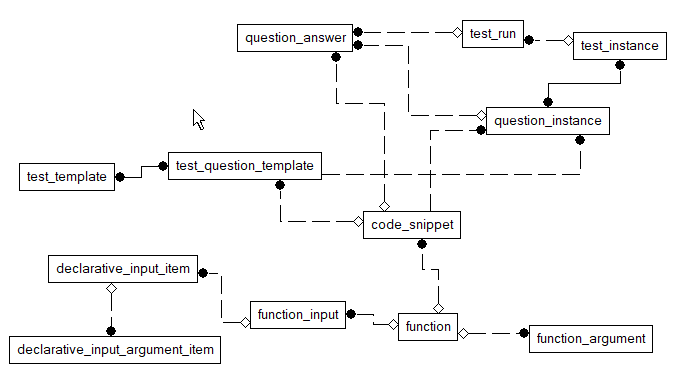
\includegraphics[width=\textwidth, center]{conceptual.png}
    \caption{Диаграмма сущность-связь}
\end{figure}
На диаграмма отображены следующие сущности:
\begin{enumerate}
    \item test\_template - Шаблон теста
    \item test\_question\_template - Шаблон вопроса
    \item code\_snippet - Объект для представления кода процедуры
    \item test\_instance - Тестовое событие
    \item question\_instance - Вопрос, принадлежащий тестовому
    событию
    \item test\_run - Прохожение тестирования
    \item question\_answer - Ответ на вопрос теста
    \item function - Процедура
    \item function\_argument - Аргумент процедуры
    \item function\_input - Набор тестовых параметров процедуры
    \item declarative\_input\_item
    \item declarative\_input\_argument\_item
\end{enumerate}

\paragraph{Связи между сущностями}
\begin{enumerate}
	\item Тестовый шаблон может иметь несколько тестовых вопросов
	\item Тестоый вопрос может принадлежать к нескольким тестам
	\item Вопрос тестового события принадлежит к одному шаблону вопроса
	\item Тестовое событие содержит несколько вопросов
	\item Ответ на вопрос принаджежит только к одному событию
	\item Функция может иметь сколько угодно аргументов,
	реализаций и тестирующих данных
\end{enumerate}

Были определены слудующие домены
\begin{figure}[H]
	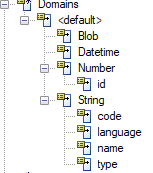
\includegraphics[center]{domains.png}
	\caption{Определенные домены}
\end{figure}
\section{Модель данных, основанная на ключах}
\begin{figure}[H]
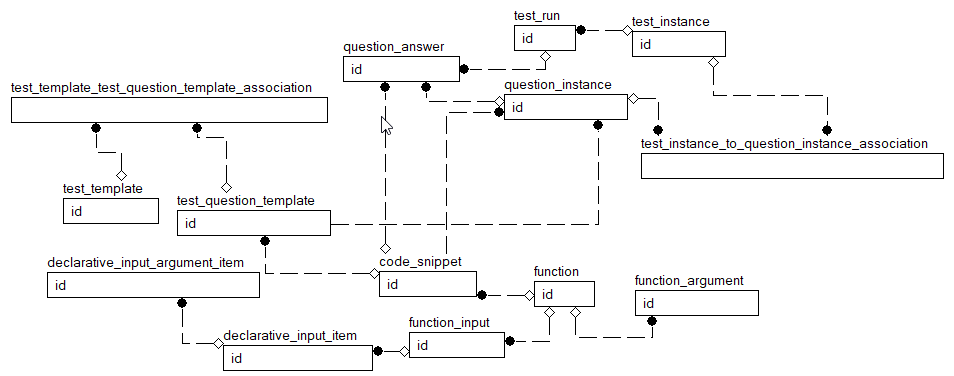
\includegraphics[width=\textwidth, center]{key_based.png}
\caption{Модель данных, основанная на ключах}
\end{figure}
На данной схеме связи типа многие-ко-многим между парами
сущностей test\_template и test\_question\_template, test\_instance и
question\_instance были заменены двумя связями, выраженными
с помощью промежуточных таблиц test\_template\_question\_template\_association
и test\_instance\_to\_question\_instance\_association.

\section{Полная аттрибутивная модель}
\begin{figure}[H]
	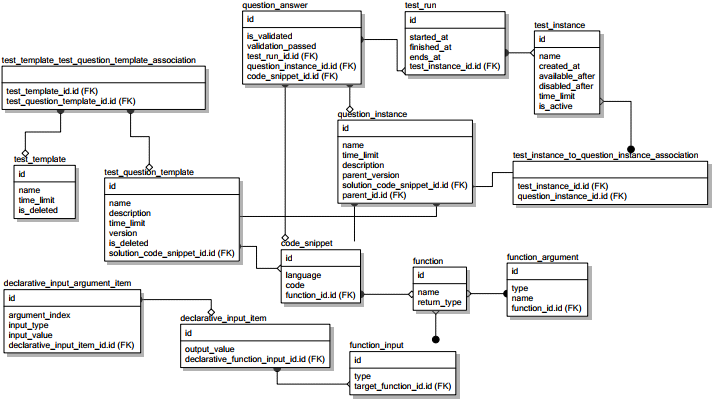
\includegraphics[width=\textwidth, center]{attr_based.png}
	\caption{Полная аттрибутивная модель}
\end{figure}

На данной модели были добавлены аттрибуты к сущностям.
\paragraph{Аттрибуты сущности test\_template}
\begin{enumerate}
	\item name - Название
	\item time\_limit - Ограничение по времени
	\item is\_deleted - Маркер удаления
\end{enumerate}

\paragraph{Аттрибуты test\_qustion\_template}
\begin{enumerate}
	\item name - Название
	\item time\_limit - Ограничение по времени
	\item is\_deleted - Маркер удаления
	\item description - Описание вопроса
	\item version - Версия вопроса
	\item solution\_code\_snippet\_id - Первичный ключа
	сущности solution\_code\_snippet  
\end{enumerate}

\paragraph{Аттрибуты сущности test\_template\_test\_question\_template\_association}
\begin{enumerate}
	\item test\_template\_id - Первичный ключ сущности
	test\_template
	\item test\_question\_template\_id - Первичный ключ сущности
	test\_question\_template
\end{enumerate}

\paragraph{Аттрибуты сущности code\_snippet}
\begin{enumerate}
	\item language - Язык программирования
	\item code - Код решения
	\item function\_id - Первичный ключ сущности function
\end{enumerate}

\paragraph{Аттрибуты сущности function}
\begin{enumerate}
	\item name - Название
	\item return\_type - Тип возвращаемого значения
\end{enumerate}

\paragraph{Аттрибуты сущности function\_argument}
\begin{enumerate}
	\item type - Типа аргумента
	\item name - Название
	\item function\_id - Первичный ключ сущности
	function
\end{enumerate}

\paragraph{Аттрибуты сущности function\_input}
\begin{enumerate}
	\item type - Дискриминатор объекта (для наследования)
	\item target\_function\_id - Первичный ключ
	сущности function
\end{enumerate}

\paragraph{Аттрибуты сущности declarative\_input\_item}
\begin{enumerate}
	\item output\_value - Ожидаемое возвращемое значение
	\item declarative\_function\_input\_id - Первичный ключ
	сущности function\_input
\end{enumerate}

\paragraph{Аттрибуты сущности declarative\_input\_argument\_item}
\begin{enumerate}
	\item argument\_index - Индекс аргумента
	\item input\_type - Тип входного параметра
	\item input\_value Входное значение
	\item declarative\_input\_item\_id - Первичный ключ сущности
	declarative\_input\_item
\end{enumerate}

\paragraph{Аттрибуты сущности question\_instance}
\begin{enumerate}
	\item name - Название
	\item time\_limit - Ограничение по времени
	\item description - Описание вопроса
	\item parent\_version - Версия вопроса
	\item parent\_id - Первичный ключ сущности
	test\_question\_template
	\item solution\_code\_snippet\_id - Первичный ключа
	сущности solution\_code\_snippet  
\end{enumerate}

\paragraph{Аттрибуты сущности test\_instance}
\begin{enumerate}
	\item name - Название
	\item time\_limit - Ограничение по времени
	\item is\_active - Маркер доступности
	\item created\_at - Дата и время создания
	\item available\_after - Дата, после которой событие
	станет доступным для прохождение
	\item disabled\_after - Дата, после которой событие
	будет завершено
\end{enumerate}

\paragraph{Аттрибуты сущности test\_run}
\begin{enumerate}
	\item started\_at - Дата и время начала прохождения теста
	\item finished\_at - Дата и время фактического завершения теста
	\item ends\_at - Дата и время ожидаемого завершения теста
	\item test\_instance\_id - Первичный ключ сущности test\_instance
\end{enumerate}

\paragraph{Аттрибуты сущности question\_answer}
\begin{enumerate}
	\item is\_validated - Был ли ответ проверен
	\item validation\_passed - Прошел ли ответ проверку
	\item test\_run\_id - Первичный ключ сущности test\_run
	\item question\_instance\_id - Первчиный ключ сущности question\_instance 
	\item code\_snippet\_id - Первичный ключ сущности code\_snipept
\end{enumerate}


\section{Трансформационная модель}
В данной модели было добавлено представление AnswerView
для отображения результатов прохождения тестирования
\begin{figure}[H]
	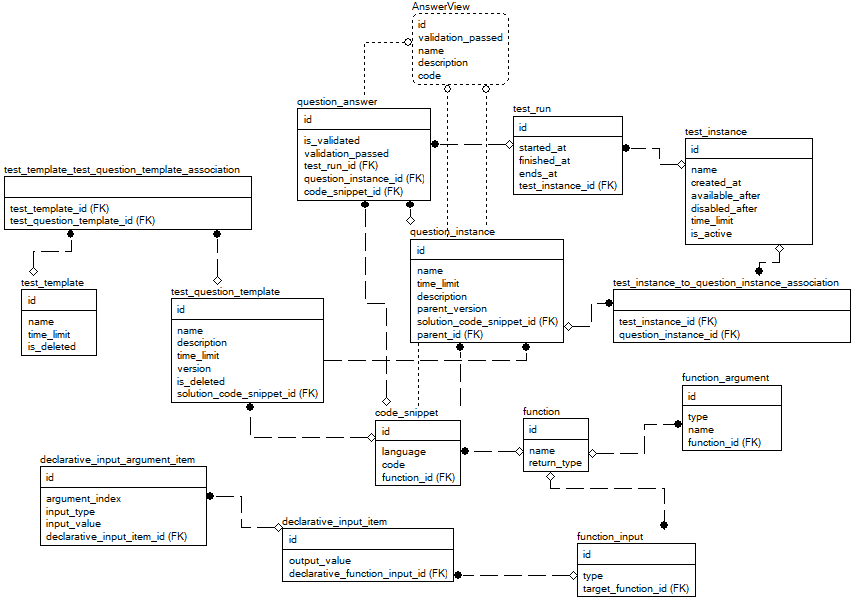
\includegraphics[width=\textwidth, center]{transformed_model.png}
	\caption{Трансформационная модель}
\end{figure}


\section{Модель СУБД}
В качестве СУБД была использована MySQL.

Для генерации созданной модели данны был получен
следующий скрипт:

\lstset{breaklines=true}
\begin{lstlisting}
 

	CREATE TABLE code_snippet
	(
		id  integer NOT NULL,
		language  INTEGER NULL,
		code  text(65535) NULL,
		function_id  integer NULL
	)
	;
	
	ALTER TABLE code_snippet
		ADD  PRIMARY KEY (id)
	;
	
	CREATE TABLE declarative_input_argument_item
	(
		id  integer NOT NULL,
		argument_index  integer NULL,
		input_type  VARCHAR(20) NULL,
		input_value  text(65535) NULL,
		declarative_input_item_id  integer NULL
	)
	;
	
	ALTER TABLE declarative_input_argument_item
		ADD  PRIMARY KEY (id)
	;
	
	CREATE TABLE declarative_input_item
	(
		id  integer NOT NULL,
		output_value  text(65535) NULL,
		declarative_function_input_id  integer NULL
	)
	;
	
	ALTER TABLE declarative_input_item
		ADD  PRIMARY KEY (id)
	;
	
	CREATE TABLE function
	(
		id  integer NOT NULL,
		name  varchar(100) NULL,
		return_type  char(13) NULL
	)
	;
	
	ALTER TABLE function
		ADD  PRIMARY KEY (id)
	;
	
	CREATE TABLE function_argument
	(
		id  integer NOT NULL,
		type  char(13) NULL,
		name  varchar(100) NULL,
		function_id  integer NULL
	)
	;
	
	ALTER TABLE function_argument
		ADD  PRIMARY KEY (id)
	;
	
	CREATE TABLE function_input
	(
		id  integer NOT NULL,
		type  varchar(50) NULL,
		target_function_id  integer NULL
	)
	;
	
	ALTER TABLE function_input
		ADD  PRIMARY KEY (id)
	;
	
	CREATE TABLE question_answer
	(
		id  integer NOT NULL,
		is_validated  tinyint NULL,
		validation_passed  tinyint NULL,
		test_run_id  integer NULL,
		question_instance_id  integer NULL,
		code_snippet_id  integer NULL
	)
	;
	
	ALTER TABLE question_answer
		ADD  PRIMARY KEY (id)
	;
	
	CREATE TABLE question_instance
	(
		id  integer NOT NULL,
		name  varchar(100) NULL,
		time_limit  integer NULL,
		description  text(65535) NULL,
		parent_version  bigint NOT NULL,
		solution_code_snippet_id  integer NOT NULL,
		parent_id  integer NOT NULL
	)
	;
	
	ALTER TABLE question_instance
		ADD  PRIMARY KEY (id)
	;
	
	CREATE TABLE test_instance
	(
		id  integer NOT NULL,
		name  varchar(100) NULL,
		created_at  datetime NULL,
		available_after  datetime NULL,
		disabled_after  datetime NULL,
		time_limit  integer NULL,
		is_active  tinyint NULL
	)
	;
	
	ALTER TABLE test_instance
		ADD  PRIMARY KEY (id)
	;
	
	CREATE TABLE test_instance_to_question_instance_association
	(
		test_instance_id  integer NULL,
		question_instance_id  integer NULL
	)
	;
	
	CREATE TABLE test_question_template
	(
		id  integer NOT NULL,
		name  varchar(100) NULL,
		description  text(65535) NULL,
		time_limit  integer NULL,
		version  bigint NULL,
		is_deleted  tinyint NULL,
		solution_code_snippet_id  integer NULL
	)
	;
	
	ALTER TABLE test_question_template
		ADD  PRIMARY KEY (id)
	;
	
	CREATE TABLE test_run
	(
		id  integer NOT NULL,
		started_at  datetime NULL,
		finished_at  datetime NULL,
		ends_at  datetime NULL,
		test_instance_id  integer NULL
	)
	;
	
	ALTER TABLE test_run
		ADD  PRIMARY KEY (id)
	;
	
	CREATE TABLE test_template
	(
		id  integer NOT NULL,
		name  varchar(100) NULL,
		time_limit  integer NULL,
		is_deleted  tinyint NULL
	)
	;
	
	ALTER TABLE test_template
		ADD  PRIMARY KEY (id)
	;
	
	CREATE TABLE test_template_test_question_template_association
	(
		test_template_id  integer NULL,
		test_question_template_id  integer NULL
	)
	;
	
	CREATE VIEW AnswerView ( id,validation_passed,name,description,code )  AS
		SELECT question_answer.id,question_answer.validation_passed,question_instance.name,question_instance.description,code_snippet.code
			FROM question_answer,question_instance,code_snippet
	;
	
	ALTER TABLE code_snippet
		ADD FOREIGN KEY code_snippet_ibfk_1 (function_id) REFERENCES function(id)
	;
	
	ALTER TABLE declarative_input_argument_item
		ADD FOREIGN KEY declarative_input_argument_item_ibfk_1 (declarative_input_item_id) REFERENCES declarative_input_item(id)
	;
	
	ALTER TABLE declarative_input_item
		ADD FOREIGN KEY declarative_input_item_ibfk_1 (declarative_function_input_id) REFERENCES function_input(id)
	;
	
	ALTER TABLE function_argument
		ADD FOREIGN KEY function_argument_ibfk_1 (function_id) REFERENCES function(id)
	;
	
	ALTER TABLE function_input
		ADD FOREIGN KEY function_input_ibfk_1 (target_function_id) REFERENCES function(id)
	;
	
	ALTER TABLE question_answer
		ADD FOREIGN KEY question_answer_ibfk_3 (code_snippet_id) REFERENCES code_snippet(id)
	;
	
	ALTER TABLE question_answer
		ADD FOREIGN KEY question_answer_ibfk_2 (question_instance_id) REFERENCES question_instance(id)
	;
	
	ALTER TABLE question_answer
		ADD FOREIGN KEY question_answer_ibfk_1 (test_run_id) REFERENCES test_run(id)
	;
	
	ALTER TABLE question_instance
		ADD FOREIGN KEY question_instance_ibfk_2 (parent_id) REFERENCES test_question_template(id)
	;

	ALTER TABLE question_instance
		ADD FOREIGN KEY question_instance_ibfk_1 (solution_code_snippet_id) REFERENCES code_snippet(id)
	;
	
	ALTER TABLE test_instance_to_question_instance_association
		ADD FOREIGN KEY test_instance_to_question_instance_association_ibfk_2 (question_instance_id) REFERENCES question_instance(id)
	;
	
	ALTER TABLE test_instance_to_question_instance_association
		ADD FOREIGN KEY test_instance_to_question_instance_association_ibfk_1 (test_instance_id) REFERENCES test_instance(id)
	;
	
	ALTER TABLE test_question_template
		ADD FOREIGN KEY test_question_template_ibfk_1 (solution_code_snippet_id) REFERENCES code_snippet(id)
	;
	
	ALTER TABLE test_run
		ADD FOREIGN KEY test_run_ibfk_1 (test_instance_id) REFERENCES test_instance(id)
	;
	
	ALTER TABLE test_template_test_question_template_association
		ADD FOREIGN KEY test_template_test_question_template_association_ibfk_2 (test_question_template_id) REFERENCES test_question_template(id)
	;
	
	ALTER TABLE test_template_test_question_template_association
		ADD FOREIGN KEY test_template_test_question_template_association_ibfk_1 (test_template_id) REFERENCES test_template(id)
	;
	
\end{lstlisting}

\begin{figure}[H]
	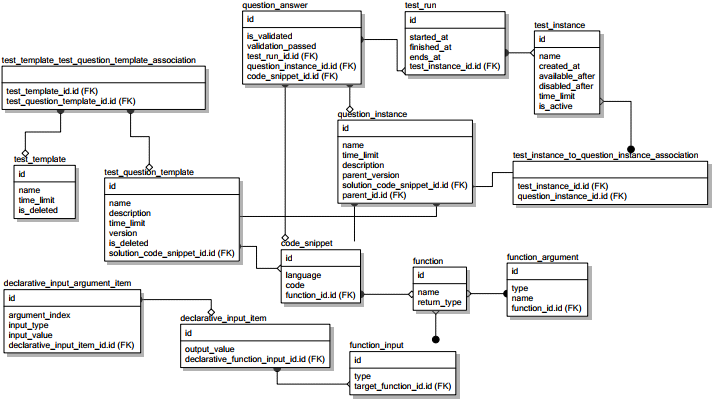
\includegraphics[width=\textwidth, center]{attr_based.png}
	\caption{Модель, полученная с помощью обратной генерации}
\end{figure}


\section{Автодокументация}
В данном разделе будут представлены отчеты, автоматически сгенерированные
с помощью ERWin.

\begin{figure}[H]
	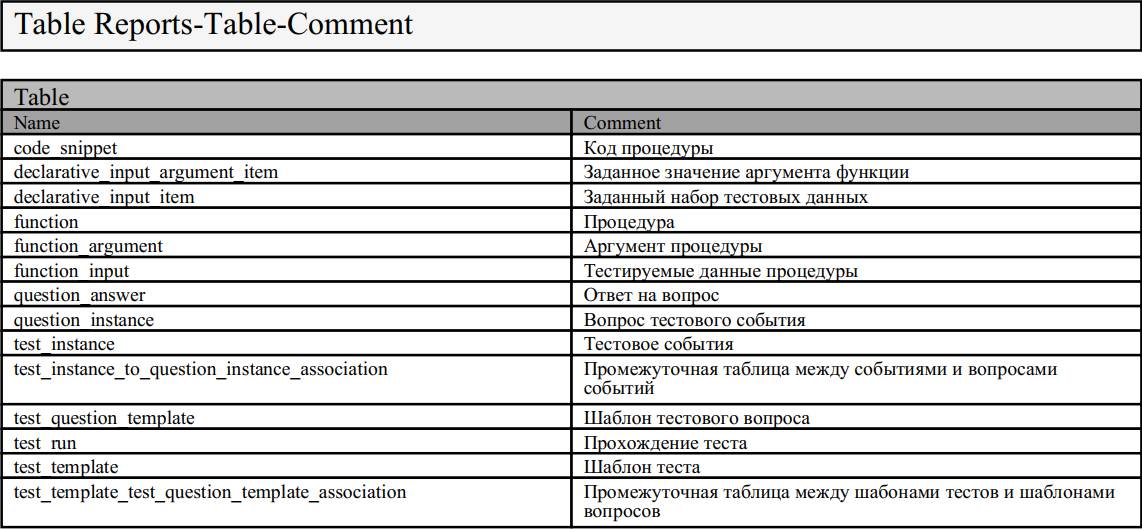
\includegraphics[width=\textwidth, center]{TableDefinitions.png}
	\caption{Отчет о созданных таблицах базы данных}
\end{figure}

\begin{figure}[H]
	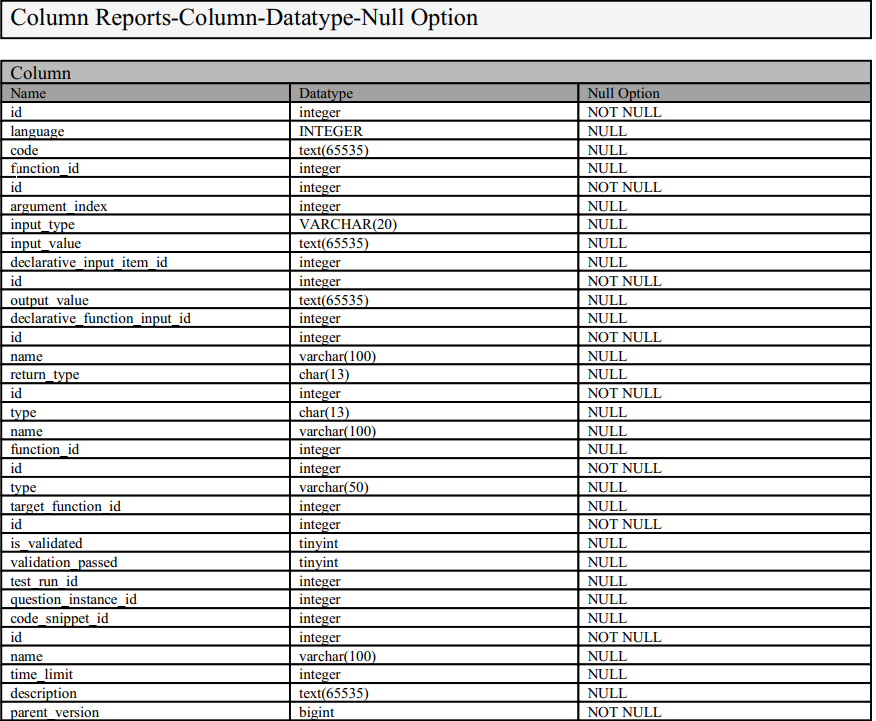
\includegraphics[width=\textwidth, center]{ColumnReport_Part1.png}
	\caption{Отчет о созданных столбцах базы данных, часть 1}	
\end{figure}

\begin{figure}[H]
	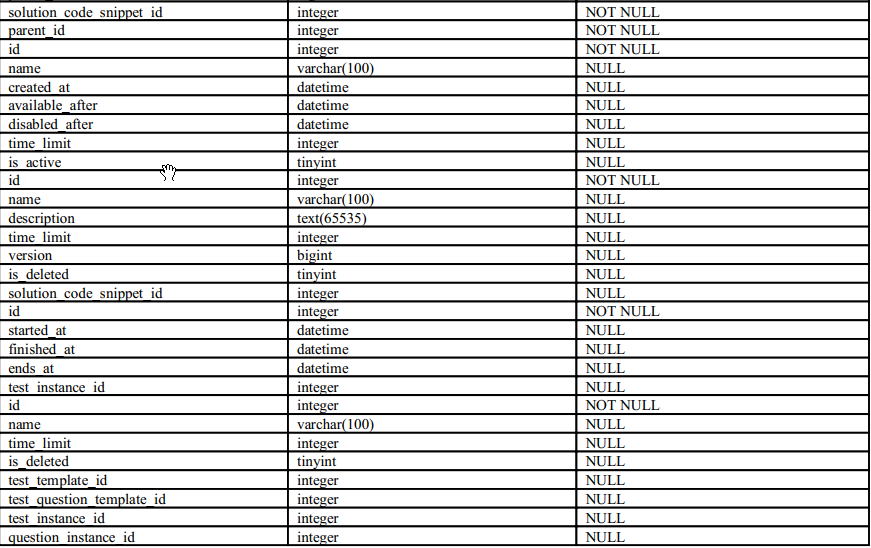
\includegraphics[width=\textwidth, center]{ColumnReport_Part2.png}
	\caption{Отчет о созданных столбцах базы данных, часть 2}	
\end{figure}

\begin{figure}[H]
	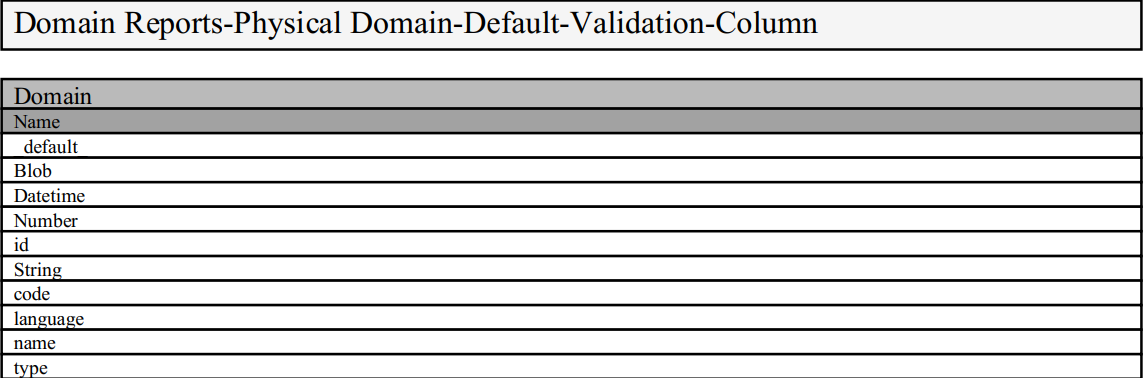
\includegraphics[width=\textwidth, center]{DefinedDomains.png}
	\caption{Отчет об определенных доменах}
\end{figure}

\begin{figure}[H]
	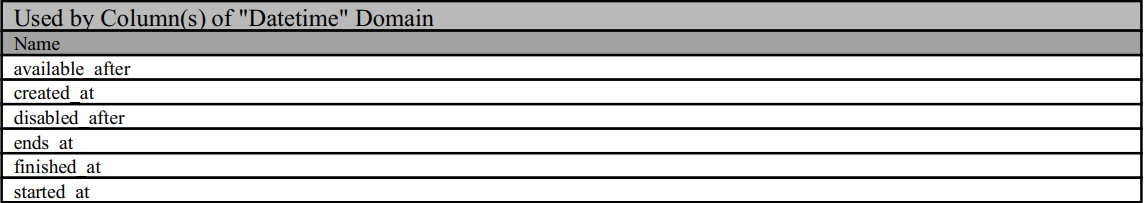
\includegraphics[width=\textwidth, center]{DateTimeDomain.png}
	\caption{Колонки, определенные на домене DateTime}
\end{figure}

\begin{figure}[H]
	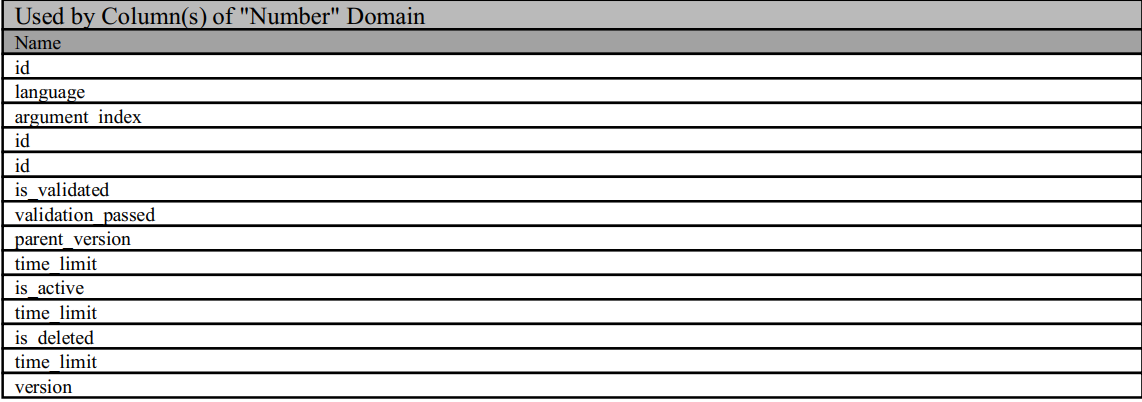
\includegraphics[width=\textwidth, center]{NumberDomain.png}
	\caption{Колонки, определенные на домене Number}
\end{figure}

\end{document}
